\documentclass[11pt]{amsbook}
\usepackage[utf8]{inputenc}
\usepackage{Ceyhun}
\usepackage{amsTurkish}
\usepackage[turkish]{babel}
\usepackage{lipsum}
\begin{document}
\hPage{3}

Her somut gösterime karşı düşen soyut bir gösterim
de bulunabileceği için, bundan böyle Ç(d,a)
çizgesinin soyut ya da somut bir gösterim olduğuna
iliskin herhangi bir ayırırnda bulunmayacağız.
Çizgede, bir düğüme bağlı olan bütün ayrıtların
oluşturduğu kümeye, o düğümün tanımladığı 
\underline{\emph{çakışım kümesi}} diyeceğiz. Örneğin, Şekil 1.1.1 deki Ç(4,5) çizgesi için \\*
\begin{center} $(a_{1},a_{2},a_{3})\quad  ,\quad  (a_{1},a_{4})\quad  ,\quad  (a_{2},a_{5})  \quad \textrm{ve} \quad (a_{3},a_{4},a_{5}) $ \end{center} 
sırasıyla $d_{1},d_{2},d_{3}  \quad \textrm{ve} \quad d_{4}$ düğümlerinin tanımladğı çakışım kümeleridir. Şekil 1.1.2 de gösterilen Ç(1,0) (\underline{\emph{tekdüğüm}}), Ç(1,1) (\underline{\emph{tekçevre}}) ve Ç(2,1) (\underline{\emph{tekayrıt}})  çizgelerine kısaca \emph{ilkel çizge} diyeceğiz ve başkaca belirtilmedikçe bu tür
çizgeler üzerinde durmayacağız. 
\begin{center}
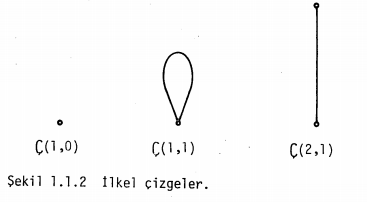
\includegraphics{images/ceyhun-3-figure-1}
\end{center}
\end{document}
Bir ayrıtın çakışık olduğu düğüm çiftine, söz.
konusu ayrıtın \underline{\emph{uc düğümleri}} diyeceğiz. Uç 
